% !TEX root =  free221.tex
\chapter{Exponentials and Logarithms (naturally)}
\label{ch:exponentials}
% !!! Issue: Limits of sequences are assumed here, but are not defined anywhere
In this chapter we first recall some facts about exponentials ($x^y$ with $x>0$
and $y$ arbitrary): they should be familiar from algebra, or ``precalculus''.
What is new is perhaps the definition of $x^y$ when $y$ is not a rational
number: for example, we know that $2^{3/4}$ is the 4th root of the third power
of 2 ($\sqrt[4]{2^3}$), but what should we take as the definition of something
like $2^{\sqrt{2}}$?

Next we ask ``what is the derivative of $f(x)=a^x$?'' The answer leads us to the
famous number $e\approx 2.718\, 281\, 828\, 459\, 045\, 235\, 360\, 287\, 471\,
352\, 662\, 497\, 757\, 247\, 093\, 699\, 95\cdots$.

Finally, we compute the derivative of $f(x)=\log_a x$, and we discuss the notion
of ``exponential growth''.


\section{Exponents} %{{{1
Here we discuss the definition of $x^y$ when $x$ and $y$ are arbitrary
real numbers, with $x>0$.




For any real number $x$ and any positive integer $n=1, 2, 3, \ldots$ one defines
\[
x^n = \overbrace{x\cdot x\cdot \cdots \cdot x}^{\text{$n$ times}}
\]
and, if $x\neq0$,
\[
x^{-n} = \frac1{x^n}.
\]
One defines $x^0=1$ for any $x\ne0$.




To define $x^{p/q}$ for a general fraction $\frac p q$ one must assume
that the number $x$ is positive. One then defines
\begin{equation}\label{eq:pqpowerofx-def}
  x^{p/q}= \sqrt[q]{x^p}.
\end{equation}
This does not tell us how to define $x^a$ is the exponent $a$ is not a fraction.
One can define $x^a$ for irrational numbers $a$ by taking limits.  For example,
to define $2^{\sqrt{2}}$, we look at the sequence of numbers obtained by truncating
the decimal expansion of $\sqrt{2}$, namely
\[
a_1 = 1,
\qquad   a_2= 1.4=\tfrac{14}{10},
\qquad    a_3=1.41=\tfrac{141}{100},
\qquad a_4= 1.414=\tfrac{1414}{1000},
\qquad   \cdots.
\]
Each $a_n$ is a rational number, so we know what $2^{a_n}$ is; for example,
$2^{a_4} = \sqrt[1000]{2^{1414}}$.  Our definition of $2^{\sqrt{2}}$ then is
\[
2^{\sqrt{ 2}} = \lim_{n\to\infty} 2^{a_n},
\]
which is to say, we define $2^{\sqrt{2}}$ as the ``limit of the sequence''
\[
2, \sqrt[10]{2^{14}}, \sqrt[100]{2^{141}}, \sqrt[1000]{2^{1414}}, \cdots
\]
(See table \ref{tbl:07twototheroottwo}.)




\begin{table}[htp]
  \begin{center}
    \begin{tabular}{ll}
      \toprule
      $x=\dfrac pq$  &  $\displaystyle 2^x = \sqrt[q]{2^p}$\\
      \midrule
      1.0000000000=$\frac11$ &
      \textbf{2}\textit{\textcolor{red}{.000000000000}}  \\[2pt]
      1.4000000000=$\frac{14}{10}$ &
      \textbf{2.6}\textit{\textcolor{red}{39015821546}}  \\[2pt]
      1.4100000000=$\frac{141}{100}$  &
      \textbf{2.6}\textit{\textcolor{red}{57371628193}}  \\[2pt]
      1.4140000000 &  \textbf{2.66}\textit{\textcolor{red}{4749650184}}  \\
      1.4142000000 &  \textbf{2.6651}\textit{\textcolor{red}{19088532}}  \\
      1.4142100000 &  \textbf{2.6651}\textit{\textcolor{red}{37561794}}  \\
      1.4142130000 &  \textbf{2.66514}\textit{\textcolor{red}{3103798}}  \\
      1.4142135000 &  \textbf{2.665144}\textit{\textcolor{red}{027466}}  \\
      $\vdots$  &\hspace{24pt} $\vdots$\\
      \bottomrule
    \end{tabular}
  \end{center}\smallskip
  \caption{Approximating $2^{\sqrt{2}}$ by computing $2^x$ for rational
numbers $x$.  Note that as $x$ gets closer to $\sqrt2$ the quantity
$2^x$ appears to converge to some number.  This limit is our
definition of $2^{\sqrt{2}}$.}
  \label{tbl:07twototheroottwo}
\end{table}%








Here one ought to prove that this limit exists, and that its value does not
depend on the particular choice of numbers $a_n$ tending to $a$. We will not go
into these details in this course.




In precalculus you learn that the exponential functions satisfy the
following properties:
\begin{equation}\label{eq:exponential-properties}
  x^a x^b = x^{a+b}, \qquad
  \dfrac{x^a}{x^b} = x^{a-b}, \qquad
  \bigl(x^a\bigr)^b = x^{ab}
\end{equation}
provided $a$ and $b$ are rational numbers. In fact these properties still
hold if $a$ and $b$ are arbitrary real numbers. Again, we
won't go through the proofs here.




Now instead of considering $x^a$ as a function of $x$ we can pick a positive
number $a$ and consider the function $f(x) = a^x$. This function is defined for
all real numbers $x$ (as long as the base $a$ is positive.).




\subsection{The trouble with powers of negative numbers. } %{{{2
The cube root of a negative number is well defined.  For instance,
$\sqrt[3]{-8}=-2$ because $(-2)^3 = -8$.  In view of the definition
\eqref{eq:pqpowerofx-def} of $x^{p/q}$ we can write this as
\[
(-8)^{1/3} = \sqrt[3]{(-8)^1} = \sqrt[3]{-8} = -2.
\]
But there is a problem: since $\frac{2}{6}=\frac13$ we might think that
$(-8)^{2/6} = (-8)^{1/3}$.  However our definition \eqref{eq:pqpowerofx-def}
tells us that
\[
(-8)^{2/6} = \sqrt[6]{(-8)^2} = \sqrt[6]{+64} =  +2.
\]
Another example:
\[
(-4)^{1/2} = \sqrt{-4} \text{ is not defined}
\]
but, even though $\frac12=\frac24$,
\[
(-4)^{2/4} = \sqrt[4]{(-4)^2}  = \sqrt[4]{+16} = 2 \text{ is defined.}
\]

There are two ways out of this mess: either
\begin{enumerate}\sffamily\itshape
\item avoid taking fractional powers of negative numbers, or
\item whenever we compute $x^{p/q}$, we first simplify the fraction by removing
  common divisors of $p$ and $q$.
\end{enumerate}
The safest option is just not to take fractional powers of negative numbers.




Given that fractional powers of negative numbers cause all these
headaches it is not surprising that we didn't try to define $x^a$ for
negative $x$ if $a$ is irrational.  For example, $(-8)^\pi$ is not
defined\footnote{There is a definition of $(-8)^\pi$ which uses complex
numbers, but we won't see or need this in the calculus sequence; it
will show up in math 319 or 320 where complex exponentials are
treated, and you will also run into $(-8)^\pi$ if you take an
electrical engineering course where ``phasors'' are discussed}.



\section{Logarithms} %{{{1
Briefly, if $a$ is a positive constant not equal to 1, then we define $y=\log_a
x$ to be the inverse function to $y=a^x$. This means that, by definition,
\[
y=\log_a x \iff x=a^y.
\]
In other words, $\log_a x$ is the answer to the question ``for which number $y$
does one have $x=a^y$?''  The number $\log_a x$ is called \emph{the logarithm of
$x$ to the base $a$}.  Note that since exponentials are always positive, the
logarithm of 0 or of a negative number is not defined\footnote{Again, there is a
way to define logarithms of negative numbers using complex numbers. We will not
pursue these ideas at the moment.}


For instance,
\[
2^3 = 8, \quad
2^{1/2} = \sqrt2,\quad
2^{-1}= \frac12
\]
so
\[
\log_2 8 = 3,\quad
\log_2\bigl(\sqrt{2}\bigr) = \frac12,\quad
\log_2 \frac12 = -1.
\]
Also:
\[
\log_2 (-3) \text{ doesn't exist}
\]
because there is no number $y$ for which $2^y = -3$ ($2^y$ is always positive)
and
\[
\log_{-3}2 \text{ doesn't exist either}
\]
because $y=\log_{-3}2$ would have to be some real number which satisfies $(-3)^y
= 2$, and we don't take non-integer powers of negative numbers.






\section{Properties of logarithms} %{{{1
In general one has
\[
\log_a a^x = x,  \text{ and }  a^{\log_a x}=x.
\]
There is a subtle difference between these formulas: the first one holds for all
real numbers $x$, but the second only holds for $x>0$, since $\log _a x$ doesn't
make sense for $x\leq 0$.




Again, you learn the following formulas in precalculus:
\begin{equation}
  \begin{aligned}
    \log_a xy &= \log_a x + \log _a y \\
    \log_a \frac xy &= \log_ax-\log_a y
  \end{aligned}
  \qquad\qquad
  \begin{aligned}
    \log_a x^y &= y\log_a x \\
    \log_a x &= \dfrac{\log_b x}{\log_b a}
  \end{aligned}
  \label{eq:07logarithm-properties}
\end{equation}
They follow from \eqref{eq:exponential-properties}, and to review this
subject it is good to write out the reason why $a^{p+q} = a^p a^q$
implies $\log_a xy = \log_a x + \log_a y$, and similarly for the other
formulas in \eqref{eq:07logarithm-properties}.




\section{Graphs of exponential functions and logarithms} %{{{1
Figure \ref{fig:07expplot} shows the graphs of some exponential
functions $y=a^x$ with different values of $a$, and Figure
\ref{fig:07logplot} shows the graphs of $y=\log_2 x$, $y=\log_3 x$,
$\log_{1/2}x$, $\log_{1/3}(x)$ and $y=\log_{10}x$.




\begin{figure}[t]\centering
  
    \begin{picture} (270.000000,140.322581)(0,0)
    \put(0.0, 0.0){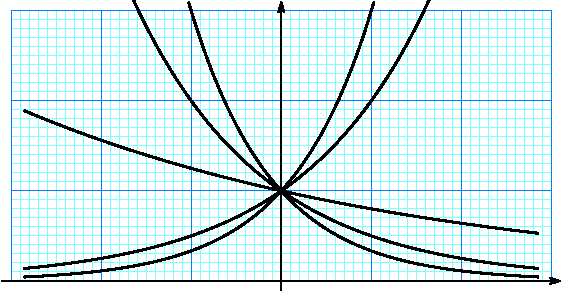
\includegraphics{07expplot.pdf}}
        \put(  3.32,  -6.68){\sffamily\itshape -3}
    \put( 46.55,  -6.68){\sffamily\itshape -2}
    \put( 89.77,  -6.68){\sffamily\itshape -1}
    \put(133.00,  -6.68){\sffamily\itshape  0}
    \put(176.23,  -6.68){\sffamily\itshape  1}
    \put(219.45,  -6.68){\sffamily\itshape  2}
    \put(262.68,  -6.68){\sffamily\itshape  3}
    \put(138.00,  88.77){\sffamily\itshape 2}
    \put(138.00, 132.00){\sffamily\itshape 3}
\end{picture}

  \caption{The graphs of $y=2^x, 3^x, (1/2)^x, (1/3)^x$ and $y=(4/5)^x$.
    The graphs are purposely not labeled: can you figure out which is which?}
  \label{fig:07expplot}
\end{figure}




From precalculus we recall:
\begin{itemize}
\item If $a>1$ then $f(x)=a^x$ is an increasing function of $x$.
\item If $0<a<1$ then $f(x)=a^x$ is a decreasing function of $x$.
\end{itemize}
In other words, for $a>1$ it follows from $x_1<x_2$ that
$a^{x_1}<a^{x_2}$; if $0<a<1$, then $x_1<x_2$ implies $a^{x_1} >
a^{x_2}$.

These statements can be shown using the properties \ref{eq:exponential-properties}.  However, we might also try to show these properties by computing the derivatives of these functions.


\section{The derivative of $a^x$ and the definition of $e$} %{{{1
To begin, we try to differentiate the function $y=2^x$:
\begin{align*}
  \frac{d}{dx}\left[ 2^x \right]
  & = \lim_{\Delta x\to0}\frac{2^{x+\Delta x}-2^x}{\Delta x} \\
  & = \lim_{\Delta x\to0}\frac{2^{x}2^{\Delta x}-2^x}{\Delta x} \\
  & = \lim_{\Delta x\to0}2^x\frac{2^{\Delta x}-1}{\Delta x} \\
  & = 2^x \lim_{\Delta x\to0}\frac{2^{\Delta x}-1}{\Delta x}.
\end{align*}




So if we assume that the limit
\[
\lim_{\Delta x\to0}\frac{2^{\Delta x}-1}{\Delta x}=C
\]
exists, then we have
\begin{equation}
  \label{eq:derivativeof2x}
  \frac{d 2^x}{dx} = C 2^x.
\end{equation}
On your calculator you can compute $\frac{2^{\Delta x}-1}{\Delta x}$
for smaller and smaller values of $\Delta x$, which leads you to
suspect that the limit actually does exist, and that $C\approx
0.693\;147\;\ldots$. One can in fact prove that the limit exists, but
we will not do this here.




\begin{figure}[!t]\centering
  
    \begin{picture} (360.000000,214.673267)(0,0)
    \put(0.0, 0.0){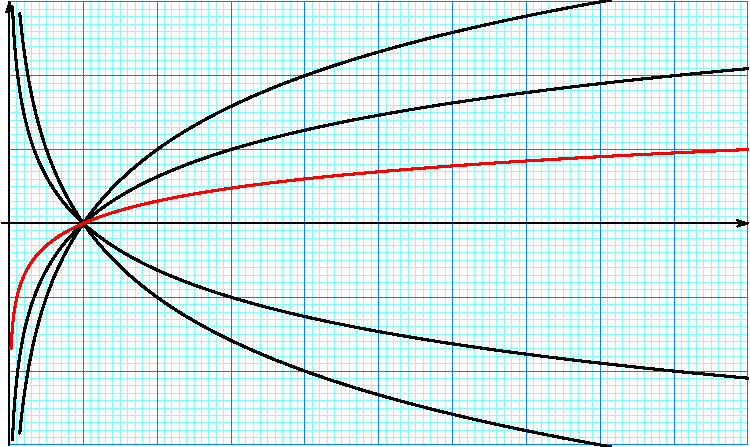
\includegraphics{07logplot.pdf}}
        \put( 37.99,  95.34){\sffamily\itshape  1}
    \put( 73.44,  95.34){\sffamily\itshape  2}
    \put(108.88,  95.34){\sffamily\itshape  3}
    \put(144.33,  95.34){\sffamily\itshape  4}
    \put(179.77,  95.34){\sffamily\itshape  5}
    \put(215.22,  95.34){\sffamily\itshape  6}
    \put(250.66,  95.34){\sffamily\itshape  7}
    \put(286.11,  95.34){\sffamily\itshape  8}
    \put(321.55,  95.34){\sffamily\itshape  9}
    \put(357.00,  95.34){\sffamily\itshape 10}
    \put( -5.46,  -2.00){\sffamily\itshape -3}
    \put( -5.46,  33.45){\sffamily\itshape -2}
    \put( -5.46,  68.89){\sffamily\itshape -1}
    \put( -5.46, 104.34){\sffamily\itshape 0}
    \put( -5.46, 139.78){\sffamily\itshape 1}
    \put( -5.46, 175.23){\sffamily\itshape 2}
    \put( -5.46, 210.67){\sffamily\itshape 3}
\end{picture}

  \caption{Graphs of some logarithms.  Each curve is the graph of a
    function $y=\log_a x$ for various values of $a>0$.  Can you tell
    what $a$ is for each graph?}
  \label{fig:07logplot}
\end{figure}








Once we know \eqref{eq:derivativeof2x} we can compute the derivative of $a^x$
for any other positive number $a$. To do this we write $a=2^{\log_2 a}$,
and hence
\[
a^x = \bigl( 2^{\log_2 a} \bigr)^x = 2^{x\cdot \log_2 a}.
\]
By the Chain Rule we therefore get
\begin{align*}
  \frac{da^x}{dx} &= \frac{d}{dx}\left[2^{x\cdot \log_2 a}\right] \\
  &= C\;2^{x\cdot \log_2 a}\; \frac{d}{dx}\left[x\cdot \log_2 a\right] \\
  &=C\;2^{x\cdot \log_2 a}\cdot \log_2 a \\
  &= (C\log_2 a) \;a^x.
\end{align*}
So the derivative of $a^x$ is just some constant times $a^x$, the constant being
$C\log_2a$.  This is essentially our formula for the derivative of $a^x$, but
one can make the formula look nicer by introducing a special number
\[
e=2^{1/C}\text{ where  }
C=\lim_{ \Delta x\to0} \frac{2^{ \Delta x} - 1}{ \Delta x}.
\]
One has
\[
e\approx 2.718\;281\;828\;459\;045\;\cdots
\]
The definition ``$e = 2^{1/C}$'' looks completely random and
unmotivated, but here is the reason why $e=2^{1/C}$ is a special
number: if you set $a=e$, then
\[
C\log_2 a = C\log_2 e = C\log_2 2^{1/C} = C\cdot \frac1C =1,
\]
and therefore the derivative of the function $y=e^x$ is
\begin{equation}
  \label{eq:derivative-of-ex}
  \frac{de^x}{dx} = e^x.
\end{equation}
Read that again: the function $e^x$ is its own derivative!




The logarithm with base $e$ is called the \emph{Natural Logarithm},
and is written
\[
\ln x = \log_e x.
\]
Thus we have
\begin{equation}
  e^{\ln x}  = x \qquad  \ln e^x = x
\end{equation}
where the second formula holds for all real numbers $x$ but the first one
only makes sense for $x>0$.




For any positive number $a$ we have $a=e^{\ln a}$, and also
\[
a^x = e^{x\ln a}.
\]
By the Chain Rule you then get
\begin{equation}
  \label{eq:derivative-of-ax}
  \dfrac{da^x}{dx} = a^x\ln a.
\end{equation}




\section{Derivatives of Logarithms} %{{{1
Since the logarithm $f(x)=\log_a x$ is the inverse function of the exponential
$g(x) = a^x$, we can find its derivative by implicit differentiation: we know
that
\[
a^{f(x)} = x.
\]
Differentiating both sides, and using the Chain Rule on the left gives
\[
(\ln a)  a^{f(x)} f'(x) = 1.
\]
Now solve for $f'(x)$ to get
\[
f'(x) = \frac{1}{(\ln a) a^{f(x)}}.
\]
Finally we remember that $a^{f(x)} = x$, and this gives us the derivative of $a^x$:
\[
\frac{da^x}{dx} = \frac{1}{x\ln a}.
\]
In particular, the natural logarithm has a very simple derivative: since $\ln
e=1$, we have
\begin{equation}\label{eq:derivative-of-ln}
 \frac{d}{dx}\left[\ln x\right] = \frac{1}{x}.
\end{equation}


\section{Limits involving exponentials and logarithms} %{{{1
\begin{theorem}  Let $r$ be any real number.  Then, if $a>1$,
  \[
  \lim_{x\to\infty} x^r a^{-x} = 0,
  \]
  i.e.
  \[
  \lim_{x \to\infty}\frac{x^r}{a^x} = 0.
  \]
\end{theorem}
This theorem says that \textit{any exponential will beat any power of $x$ as
  $x\to\infty$}.  For instance, as $x \to\infty$ both $x^{1000}$ and $(1.001)^x$
go to infinity, but
\[
\lim_{x \to\infty} \frac{x^{1000}}{(1.001)^x} = 0,
\]
so, in the long run, for very large $x$, $1.001^x$ will be much larger than
$1000^x$.


% !!! Discuss: Instead we could just repeatedly use L'Hopital's rule at
% infinity. That proof is much less horrible.

% l'Hopital's rule was not proved for f/g where f, g\to\infty.
% The rule also encourages not thinking about "how large function are"
% Its use should be discouraged.  This section should be modified to include the
% list of functions in their natural magnitude
%               (log << powers of x << exponential functions)
%

\begin{proof}[Proof when $a=e$]
  We want to show $\lim_{x\to\infty} x^re^{-x} = 0$.  To do this consider the
  function $f(x) = x^{r+1}e^{-x}$.  Its derivative is
  \[
  f'(x) = \frac{dx^{r+1}e^{-x}}{dx}
  = \bigl((r+1)x^r - x^{r+1}\bigr)e^{-x}
  = (r+1-x)x^re^{-x}.
  \]
  Therefore $f'(x) < 0$ for $x>r+1$, i.e.\ $f(x)$ is decreasing for $x>r+1$.
  It follows that $f(x) <f(r+1)$ for all $x>r+1$, i.e.
  \[
  x^{r+1}e^{-x} < (r+1)^{r+1}e^{-(r+1)}\text{ for } x>r+1.
  \]
  Divide by $x$, abbreviate $A=(r+1)^{r+1}e^{-(r+1)}$, and we get
  \[
  0<x^re^{-x}<\frac Ax \text{ for all }x>r+1.
  \]
  The Sandwich Theorem implies that $\lim_{x\to\infty} x^re^{-x} = 0$, which
  is what we had promised to show.

The case with general $a$ follows after a substitution:  given $a$ we set 
\[
 x=\frac{t}{\ln a}. 
\]
Then, since $a>1$ we have $\ln a>0$ so that as $x\to\infty$ one also has $t\to\infty$.  Therefore
\[
 \lim_{x\to\infty}
 \frac{x^r}{a^x}
 = 
 \lim_{x\to\infty}
 \frac{x^r}{e^{x\ln a}}
 = 
 \lim_{t\to\infty}
 \frac{(t/\ln a)^r}{e^{t}}
 = \underbrace{(\ln a)^{-r}}_{\textsf{constant}}\cdot 
 \underbrace{\lim_{t\to\infty}
 \frac{t^r}{e^{t}}}_{=0}
 =0.
\]


\end{proof}




\subsection{Related limits} %{{{2
If $a$, $m$, and $r$ are constants, then
\begin{subequations}
  \begin{align}
    a>1 \implies &
    \lim_{x \to\infty} \frac{a^x}{x^r} = \infty \quad(D.N.E.)
    \label{eq:07exp-beats-power-limit}\\
    m>0 \implies & \lim_{x \to\infty} \frac{\ln x}{x^m} =0
        \label{eq:07power-beats-log-atinfty-limit}\\
    m>0 \implies & \lim_{x \to 0} x^m\ln x =0
        \label{eq:07power-beats-log-atzero-limit}
  \end{align}
\end{subequations}
The second limit (\ref{eq:07power-beats-log-atinfty-limit}) says that even
though $\ln x$ becomes infinitely large as $x \to\infty$, it is always much less
than any power $x^m$ with $m>0$ real.  To prove it you set $x=e^t$ and then
$t=s/m$, which leads to
\[
\lim_{x \to\infty} \frac{\ln x}{x^m}
\;\stackrel{x=e^t}{=}\;
\lim_{t \to\infty} \frac{t}{e^{mt}}
\;\stackrel{t = s/m}{=}\;
\frac1m\;\lim_{t \to\infty}\frac{s}{e^s} = 0.
\]
The limit (\ref{eq:07power-beats-log-atzero-limit}) follows from the second by
substituting $x=1/y$ and using $\ln\frac1x = -\ln x$.




\section{Exponential growth and decay} %{{{1
\subsection{Absolute and relative growth rates} %{{{2
If a quantity $X(t)$ changes with time, then the change in $X$ during a short
time interval of length $\Delta t$ is
\[
\Delta X = X(t+\Delta t) - X(t).
\]
If $X$ is measured in certain units, then the change $\Delta X$ has
the same units as $X$.  The change $\Delta X$ is sometimes called the
\emph{absolute change}, to distinguish it from the \emph{relative
  change,} which is defined as
\[
\text{Relative change in $X$ }= \frac{\Delta X} {X}.
\]
No matter what units $X$ is measured in, the relative change has no
units and can be expressed as a percentage.  For instance, if the
population $X$ of a city increases from $200,000$ to $250,000$
(people), then the absolute population change is $50,000$ (people),
but the relative population change is
\[
\frac{50,000\text{ people}}
{200,000\text{ people}} =
\frac{1} {4} = 25\%.
\]
Just as we defined the rate of change of a quantity $X(t)$ to be
\[
\frac{dX} {dt} = \lim_{\Delta t\to0} \frac{\Delta X} {\Delta t},
\]
we define the \emph{relative rate of change} or \emph{relative growth
  rate} to be
\[
\lim_{\Delta t \to 0}
\frac{\left\{
    \parbox{90pt}{\sffamily\centering%
      Relative change in $X$\\
      from $t$ to $t+\Delta t$ }
  \right\}} {\Delta t}
= \lim_{\Delta t \to 0} \frac{\Delta X} {X \Delta t}
= \frac{1} {X}\frac{dX} {dt}.
\]




\subsection{Theorem on constant relative growth} %{{{2
\label{sec:07const-relative-growth}
\itshape%
Suppose that a time-dependent quantity $X(t)$ has a constant relative
growth rate, meaning that
\begin{equation}
  \frac{1} {X} \frac{dX} {dt} = k \text{ is constant.}
  \label{eq:07constant-relative-growth}
\end{equation}
And suppose that at time $t_0$ the value of $X$ is known to be
$X(t_0) = X_0$.  Then
\begin{equation}\label{eq:07exponentialgrowth}
  X(t) = X_0 e^{k(t-t_0)}.
\end{equation}
\upshape



% !!! Issue: The proof assumes the result that a function with zero derivative is constant! This does not appear in the text anywhere.
\begin{proof}
  The constant relative growth rate condition
  \eqref{eq:07constant-relative-growth} implies
  \begin{equation}\label{eq:07exp-growth-diffeq}
    \frac{dX(t)}{dt} = kX(t).
  \end{equation}
  The trick is to look at the rate of change of $e^{-kt}X(t)$:
  \begin{align*}
    \frac{dX(t)e^{-kt}}{dt}
    &=X(t)\frac{de^{-kt}}{dt} + \frac{dX(t)}{dt}e^{-kt}\\
    &=-kX(t) e^{-kt}+X'(t)e^{-kt}\\
    &= (X'(t) - kX(t))e^{-kt} \\
    &=0.
  \end{align*}
  In other words $X(t)e^{-kt}$ does not depend on $t$.  Therefore
  \[
  X(t)e^{-kt} = X(t_0) e^{-kt_0} = X_0 e^{-kt_0}, \text{ for any $t$.}
  \]
  Multiply with $e^{kt}$ and we end up with
  \[
  X(t) = X_0e^{k(t-t_0)}.
  \]
\end{proof}
The equations \eqref{eq:07constant-relative-growth} and
\eqref{eq:07exp-growth-diffeq} are examples of \textit{differential
  equations}.  They are equations in which the unknown quantity $X$ is
not a number but a function, and in which the derivative of the
unknown function appears.  We have just reasoned that any function
that satisfies \eqref{eq:07constant-relative-growth} (has constant
relative growth) must be of the form \eqref{eq:07exponentialgrowth}:
we have solved the differential equation\footnote{The trick we used here is an
example of solving differential equations by multiplying with an ``integrating
factor''.  We will do this more systematically in Math 222.}.




\subsection{Examples of constant relative growth or decay} %{{{2
\label{sec:07examples-of-const-relative-growth}
Here is a typical scenario of constant relative growth or, rather,
decay.  Suppose that the molecules of a certain chemical substance
appear in two varieties, the ``normal'' kind A, and the ``excited''
kind A$^*$.  Left to themselves the normal kind of molecules A are
stable, but the excited kind will randomly decay to the normal kind.
In the long run all A$^*$ will be converted into regular A molecules.
One example of this kind of reaction is radioactive decay where, say,
\raisebox{-3pt}{\footnotesize14}C decays to
\raisebox{-3pt}{\footnotesize14}N.  There are \textit{many} other
similar examples.




{\itshape%
  How fast does the conversion from {\upshape A}$^*$ to {\upshape A}
  happen?}  A very common reasoning to find the conversion rate goes
like this.  Suppose $X(t)$ is the total amount of A$^*$ and suppose
that during a short time interval of length $\Delta t$ a certain
number of conversions from A$^*$ to A take place.  If the time
interval is short, then the number of conversions will be small, and
the total amount $X(t)$ of A$^*$ molecules will not change much.
Therefore, during the next short time interval of length $\Delta t$
you would expect the same number of conversions to happen.  Adding
these together you conclude that if you wait twice as long ($2\Delta
t$) then the number of conversions doubles; more generally, you would
expect the number of conversions during a short time interval of
duration $\Delta t$ to be proportional to $\Delta t$.




If on the other hand you fix the length of the time interval, but
double the amount of A$^*$ molecules, you would expect twice as many
conversions to occur, so, the number of conversions from A$^*$ to A
during some short time interval $\Delta t$ should also be proportional
with the amount of A$^*$ present.
\marginpar{\sffamily\footnotesize%
  To say that a reaction takes place in which A$^*$ decays
  to A you could write:\\
\centerline{A$^* \stackrel{k}\longrightarrow$ A.}\\
The $k$ above the arrow is the ``reaction rate.''  }


Putting this together, we see that the change in the amount of A$^*$
during a time interval of length $\Delta t$ should be proportional
both with $X$ and with $\Delta t$, so
\[
\Delta X \approx - k\cdot X\cdot \Delta t,
\]
for some constant $k$.  The approximation should be better as you make
the time interval shorter, and therefore, dividing by $X\Delta t$ and
taking the limit $\Delta t\to0$, we see that the amount of $X$ should
satisfy
\[
\frac{1} {X} \frac{dX} {dt} = -k,
\]
which is \eqref{eq:07constant-relative-growth}, but with $k$ replaced
by $-k$.  The conclusion is: if you know that at time $t_0$ the
amount of A$^*$ is $X(t_0) = X_0$, then at any other time $t$,
\[
X(t) = X_0 e^{-k(t-t_0)}.
\]








\subsection{Half time and doubling time. } %{{{2
If $X(t) = X_0 e^{kt}$ then one has
\[
X(t+T) = X_0e^{kt+kT} = X_0e^{kt}e^{kT} = e^{kT}X(t).
\]
In words, after a time $T$ goes by, an exponentially growing (decaying) quantity
changes by a factor $e^{kT}$.  If $k>0$, so that the quantity is actually
growing, then one calls
\[
T = \frac{\ln 2}{k}
\]
the \emph{doubling time} for $X$ because $X(t)$ changes by a factor $e^{kT} =
e^{\ln2} = 2$ every $T$ time units:  $X(t)$ doubles every $T$ time units.




If $k<0$ then $X(t)$ is decaying and one calls
\[
T = \frac{\ln 2}{-k}
\]
the \emph{half life} because $X(t)$ is reduced by a factor $e^{kT} = e^{-\ln 2}
= \frac12$ every $T$ time units.




\subsection{Determining $X_0$ and $k$. } %{{{2
The general exponential growth/decay function \eqref {eq:07exponentialgrowth}
contains only two constants, $X_0$ and $k$, and if you know the values of $X(t)$
at two different times then you can compute these constants.

Suppose that you know
\[
X_1 = X(t_1) \text{ and } X_2=X(t_2).
\]
Then we have
\[
X_0e^{kt_1} = X_1 \text{ and } X_2 = X_0e^{kt_2}
\]
in which $t_1, t_2, X_1, X_2$ are given and $k$ and $X_0$ are unknown.  
One first finds $k$ from
\[
\frac{X_1}{X_2}= \frac{X_0e^{kt_1}}{X_0e^{kt_2}}
=e^{k(t_1-t_2)}
\implies \ln\frac{X_1}{X_2}= k(t_1-t_2)
\]
which implies
\[
k = \frac{\ln X_1 - \ln X_2}{t_1-t_2}.
\]
Once you have computed $k$ you can find $X_0$ from
\[
X_0 = \frac{X_1}{e^{kt_1}} = \frac{X_2}{e^{kt_2}}.
\]
(both expressions should give the same result.)
















\section{Problems} %{{{1
\problemfont %{{{3




\begin{multicols}{2}
\noindent\textbf{Sketch the graphs} of the following functions.
You should
\begin{list}{--}{
    \setlength{\itemindent}{0pt}
    \setlength{\leftmargin}{6pt}}
\item find where $f$, $f'$ and $f''$ are positive or negative
\item find all stationary points and classify them as local minima, maxima, or neither
\item find any global maxima or minima, if they exist
\item find all inflection points
\item determine all intervals where the function is increasing or decreasing
\item determine all intervals where the function is convex or concave
\item find any horizontal, vertical, or slant asymptotes
\end{list}



(\textit{Hint for some of these:  if you have to solve something like
  $e^{4x}-3e^{3x}+e^x = 0$, then call $w=e^x$ to get a polynomial
  equation $w^4-3w^3+w=0$ for $w$.})




\problem $\DS y= e^x $ %{{{3




\problem $\DS y= e^{-x} $ %{{{3




\problem $\DS y= e^{x}+e^{-2x} $ %{{{3
\answer %{{{3
$dy/dx = e^x - 2e^{-2x}$. Local min at $x = \frac13 \ln 2$.




$d^2y/dx^2 = e^x+4e^{-2x}>0$ always, so the function is convex.




$\lim_{x\to\pm\infty} y=\infty$, no asymptotes.
\endanswer




\problem $\DS y= e^{3x}-4e^x $ %{{{3
\answer %{{{3
$dy/dx = 3e^{3x} - 4 e^x$. Local min at $x=\frac12\ln\frac43$.




$d^2y/dx^2 = 9e^{3x} - 4e^{x}$ changes sign when $e^{2x} = \frac49$,
i.e.~at $x=\frac12\ln\frac49 = \ln\frac23 = \ln2-\ln3$.  Inflection
point at $x=\ln2-\ln 3$.




$\lim_{x\to-\infty}f(x) = 0$ so negative $x$ axis is a horizontal
asymptote.




$\lim_{x\to\infty}f(x) = \infty$\ldots no asymptote there.
\endanswer




\problem $\DS y= \frac{e^x}{1+e^x} $ %{{{3




\problem $\DS y= \frac{2e^x}{1+e^{2x}} $ %{{{3




\problem $\DS y= xe^{-x} $ %{{{3




\problem $\DS y= \sqrt{x}e^{-x/4} $ %{{{3




\problem $\DS y= x^2 e^{x+2} $ %{{{3




\problem $\DS y= e^{x/2}-x$ %{{{3




\problem $\DS y= \ln \sqrt x $ %{{{3




\problem $\DS y= \ln \frac1 x $ %{{{3




\problem $\DS y= x\ln x $ %{{{3




\problem $\DS y= \frac{-1}{\ln x}  \quad(0<x<\infty, x\neq1)$ %{{{3




\problem $\DS y= (\ln x)^2  \quad(x>0)$ %{{{3




\problem $\DS y= \frac{\ln x}{x} \quad(x>0)$ %{{{3




\problem $\DS y=\ln \sqrt{\frac{1+x}{1-x}} \quad(|x|<1)$ %{{{3




\problem $\DS y= \ln \bigl(1+x^2\bigr) $ %{{{3




\problem $\DS y= \ln \bigl(x^2-3x+2\bigr) \quad (x>2) $ %{{{3




\problem $\DS y= \ln\cos x\quad (|x|< \tfrac{\pi}{2})$ %{{{3




\problem $\DS y = \sqrt{e^{2x}}$ %{{{3




\problem The function $f(x) = e^{-x^2}$ plays a central role in %{{{3
statistics and its graph is called \emph{the bell curve} (because of its
shape).  Sketch the graph of $f$.




\problem Sketch the part of the graph of the function %{{{3
\[
f(x) = e^{-\frac1x}
\]
with $x>0$.
Find the limits
\[
\lim_{x\searrow 0} \frac{f(x)}{x^n}
\text{ and }
\lim_{x \to\infty} f(x)
\]
where $n$ can be any positive integer. (Hint: substitute $y=1/x$.)

\problem A \emph{damped oscillation} is a function of the form %{{{3
\[
f(x) = e^{-ax} [\cos b(x-c)]
\]
where $a$, $b$, and $c$ are constants.

\subprob $g(x) = e^{-x} \sin 10x$ is a damped oscillation.  What are
the constants $a$, $b$, and $c$?

\subprob Draw the graphs of $y=e^{-x}$, $y=-e^{-x}$, and $y=g(x)$
in one sketch (with pencil and paper).  Make sure you include the
piece of the graph with $0\leq x\leq 2\pi$.

\subprob $y=g(x)$ has many local maxima and minima.  
\textit{What is the ratio between the function values at two consecutive
  local maxima?}  (Hint: the answer does not depend on which pair of
consecutive local maxima you consider.)


\problem Find the inflection points on the graph of $f(x) = (1+x)\ln x$, for $x>0$. %{{{3



\problem \textbf{(a)~}If $x$ is large, which is bigger: $2^x$ or $x^2$?\\ %{{{3
\textbf{(b)~}The graphs of $f(x) = x^2$ and $g(x) = 2^x$ intersect at $x=2$
(since $2^2=2^2$).  How many more intersections do these graphs have (with
$-\infty < x < \infty$)?




\bigskip
\textbf{Find the following limits.}
\begin{multicols}{2}
\problem  $\DS\lim_{x\to\infty}\frac{e^x-1}{e^x+1} $ %{{{3




\problem  $\DS\lim_{x \to\infty}\frac{e^x-x^2}{e^x+x} $ %{{{3




\problem  $\DS\lim_{x\to\infty}\frac{2^x}{3^x-2^x} $ %{{{3




\problem  $\DS\lim_{x \to\infty}\frac{e^x-x^2}{e^{2x}+e^{-x}} $ %{{{3




\problem  $\DS\lim_{x \to\infty}\frac{e^{-x}-e^{-x/2}}{\sqrt{e^x+1}} $ %{{{3




\problem  $\DS\lim_{x \to\infty}\frac{\sqrt{x+e^{4x}}}{e^{2x}+x} $ %{{{3




\problem  $\DS\lim_{x \to\infty}\frac{e^{\sqrt x}}{\sqrt{e^x}} $ %{{{3




\problem  $\DS\lim_{x \to \infty} \frac{e^{\sqrt{x}}} {\sqrt{e^x+1}}$ %{{{3




\problem  $\DS\lim_{x \to\infty}\frac{\ln x}{\ln (x^2)} $ %{{{3




\problem  $\DS\lim_{x \to 0} x\ln x$ %{{{3




\problem  $\DS\lim_{x\to\infty}\frac{\ln x}{\sqrt x+\ln x} $ %{{{3




\problem  $\DS\lim_{x\to 0}\frac{\ln x}{\sqrt x+\ln x} $ %{{{3




\end{multicols}
\problem  $\DS\lim_{x \to\infty}\ln (1+x) - \ln x$ %{{{3








\problem  Find the tenth derivative of $xe^x$.  Then find the $99$th %{{{3
derivative of $xe^{x}$.




\problem For which real number $x$ is $2^x- 3^x$ the largest? %{{{3








\problem Find $\DS\frac{dx^x}{dx} $, $\DS\frac{d x^{x^x}}{dx}$, and %{{{3
$\DS\frac{d(x^x)^x}{dx} $.




\null\hfill Hint: write $x^x$ as $e^{\text{something}}$.







% !!! Issue: The other problems on logarithmic differentiation should be moved here and combined, into an actual explanation of the technique.
\problem \groupproblem \textit{About logarithmic differentiation -- %{{{3
see Problem \ref{ex:05log-derivs}.}




\subprob  Let $y=(x+1)^2(x+3)^4(x+5)^6$ and $u=\ln y$.  Find $du/dx$. Hint:
Use the fact that $\ln$ converts multiplication to addition before you
differentiate.  It will simplify the calculation.




\subprob  Check that the derivative of $\ln u(x)$ is the logarithmic
derivative of the function $u$.












\problem After $3$ days a sample of radon-222 decayed to $58\%$ of its original %{{{3
amount.

\subprob What is the half-life of radon-222?

\subprob How long would it take the sample to decay to $10\%$ of its
original amount?

\problem   Polonium-210 has a half-life of $140$ days. %{{{3

\subprob If a sample has a mass of $200$mg, find a formula for the
mass that remains after $t$ days.

\subprob Find the mass after 100 days.

\subprob When will the mass be reduced to 10 mg?

\subprob Sketch the graph of the mass as a function of time.








% \problem %{{{3
% Current agricultural experts believe that the world's farms can feed about
% 10 billion people.  The 1950 world population was 2.517 billion and the 1992
% world population was 5.4 billion.  When can we expect to run out of food?








% \problem \groupproblem The AC\textit{ME} company runs two ads on %{{{3
% Sunday mornings. One says
% that ``when this baby is old enough to vote, the world will have one
% billion new mouths to feed'' and the other says ``in thirty six years,
% the world will have to set eight billion places at the table.''  What
% does AC\textit{ME} think the population of the world is at present?
% How fast does AC\textit{ME} think the population is increasing?  Use
% units of billions of people so you  can write $8$ instead of
% $8,000,000,000$.  (Hint: $36=2\times 18$.)








% \problem The population of California grows exponentially at an instantaneous %{{{3
% rate of 2\% per year.  The population of California on January 1,
% 2000 was 20,000,000.




% \subprob Write a formula for the population $N(t)$ of California
% $t$ years after January 1, 2000.




% \subprob Each Californian consumes pizzas at the rate of 70
% pizzas per year.  At what rate is California consuming pizzas $t$
% years after 1990?




% \subprob How many pizzas were consumed in California from January
% 1, 2005 to January 1, 2009?

\problem Here are three versions of the same problem (read all \& choose one): %{{{3

\subprob The number of individuals of an endangered species decreases to half
its size every $1000$ days.  How long does it take for the population to
decrease to $75\%$ of its current size?

\subprob A radioactive substance has a half-life of $1000$ years.  How long does
it take for $25\%$ of it to decay?

\subprob The concentration of gas released in a chamber has a half-life of
$1000$ seconds. How long it would take for the gas to lower its concentration to
$75\%$ of its initial level?

\problem The remains of an old campfire are unearthed and it is found that there %{{{3
is only $80\%$ as much radioactive carbon-14 in the charcoal samples from the
campfire as there is in modern living trees.  If the half-life of carbon-14 is
$5730$ years, how long ago did the campfire burn?


\problem Max needs 1 gram of Kryptonite to perform an important experiment. %{{{3
Unfortunately, he doesn't have the lab set up for his experiment yet and his
Kryptonite is decaying.  Yesterday there were 15 grams of Kryptonite left and
today there are only 12 grams left.  How long does he have before he won't
have enough Kryptonite left to do his experiment?

\problem Two equivalent problems -- read them and pick one: %{{{3
% This problem requires a(n easy) substitution to solve, which is probably too hard.



\subprob ({\it Newton's law of cooling})
Newton's law of cooling states that the rate of change of temperature $T$
of an object is proportional to the difference between its temperature
and the ambient temperature, $U$, that is,
\[
  \frac{dT}{dt}=k\left(U-T(t)\right).
\]




A body is discovered at $7$ am. Its temperature is then $25^{\circ}$ C. By the
time police arrives at the site, at $8$ pm, the body has cooled at $20^{\circ}$
C. Assuming the normal body temperature in humans is $37^{\circ}$ C, and that
the ambient temperature is $5^{\circ}$ C, determine the time of death.




\subprob A nuclear reactor was shut down for maintenance repairs. The rate of
change of temperature in the fuel rods of the reactor is described by Newton's
law of cooling:
\[
  \frac{dT}{dt}=k\left(U-T(t)\right),
\]
where $U=5^{\circ}$ C is the temperature of the water being pumped into the
reactor. The normal temperature of the fuel rods in a working reactor is
$37^{\circ}$ C.  If at $7$ am, the temperature of fuel rods was $25^{\circ}$ C,
and an hour later the fuel rods have cooled at $20^{\circ}$ C, when was the
reactor shut down?




\problem A bacteria population grows exponentially with growth rate $k=2.5$. How %{{{3
long it will take for the bacteria population to double its size?




\problem Three equivalent problems -- read all and do one: %{{{3




\subprob The half-life of a certain drug in the human body is $8$ hours. How
long it would take for a dose of this drug to decay to $0.1\%$ of its initial
level?




\subprob After a nuclear plant explosion, radioactive material is scattered in
the atmosphere. Particularly dangerous for human health is the iodine-131,
whose half-life is $8$ days. How long it would take for the iodine-131 in the
atmosphere to decay to $0.1\%$ of its initial level?




\subprob The concentration of gas released in a chamber has a half-life of $8$
minutes. How long it would take for the gas to lower its concentration to
$0.1\%$ of its initial level?




\problem The \textit{hyperbolic functions} are defined by %{{{3
\begin{gather*}
  \sinh x = \frac{e^x-e^{-x}}2,\\
  \cosh x = \frac{e^x+e^{-x}}2,\\
  \tanh x = \frac{\sinh x}{\cosh x}.
\end{gather*}
\subprob Prove the following identities:
\begin{gather*}
  \cosh^2 x -\sinh^2 x = 1\\
  \cosh 2x = \cosh^2x + \sinh ^2 x \\
  \sinh 2x = 2\sinh x \cosh x.
\end{gather*}
\subprob Show that
\begin{gather*}
  \frac{d\sinh x}{dx} = \cosh x, \\
  \frac{d\cosh x}{dx} = \sinh x, \\
  \frac{d\tanh x}{dx} = \frac1{\cosh^2 x}.
\end{gather*}
\subprob Sketch the graphs of the three hyperbolic functions.








\problem Sketch the following parametrized curves %{{{3
(first review Chapter~V, \S\ref{sec:05parametrized-curves-and-lHopital}):




\subprob \(x(t) =  e^t \), \(y(t) = e^t  \)
\answer %{{{3
The diagonal $y=x$ again, but since $x=e^t$ can only be positive we only get the
part in the first quadrant.  At $t=-\infty$ we start at the origin, as
$t\to+\infty$ both $x$ and $y$ go to $+\infty$.
\endanswer




\subprob \(x(t) =  e^t \), \(y(t) = t  \)
\answer %{{{3
The graph of $y=\ln x$, or $x=e^y$ (same thing), traversed in the upwards
direction.
\endanswer




\subprob \(x(t) =  e^t \), \(y(t) = e^{-t}  \)
\answer %{{{3
The part of the graph of $y=1/x$ which is in the first quadrant, traversed from
left to right.
\endanswer




\problem \subprob At which point on the graph of $y=e^x$ is the %{{{3
curvature the largest?




\subprob At which point on the graph of $y=\ln x$ is the
curvature the largest?

\end{multicols}
\noproblemfont


%%% Local Variables:
%%% mode: latex
%%% TeX-master: "free221"
%%% End:
